\noindent\textbf{1.} Bên trong vật dẫn, điện trường bằng không. Các được sức phải vuông góc với mặt khoét. Do sự tích tụ các điện tích mặt, cường độ điện trường ở phía bên phải điện tích sẽ mạnh hơn phía bên trái do đó mật độ đường sức bên phải sẽ lớn hơn. Cuối cùng, lưu ý rằng điện tích là dương, các đường sức phải hướng ra ngoài điện tích. Với những lập luận trên, ta có thể phác hoạ các đường sức như hình 1.1:
\begin{figure}[h]
  \centering
  \begin{subfigure}[b]{0.49\textwidth}
    \centering
    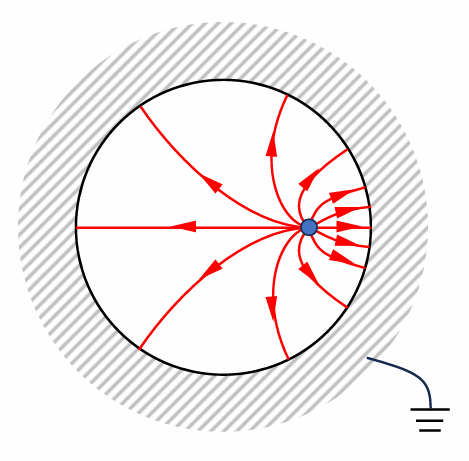
\includegraphics[width=0.75\textwidth]{Figures/Solutions/Fig 3.1.png}
    \begin{center}
      \figurename{ 3.1}
    \end{center}
  \end{subfigure}
  \hfill
  \begin{subfigure}[b]{0.49\textwidth}
    \centering
    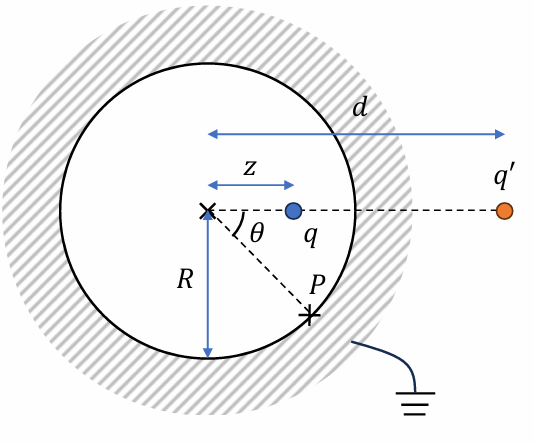
\includegraphics[width=0.85\textwidth]{Figures/Solutions/Fig 3.2.png}
    \begin{center}
      \figurename{ 3.2}
    \end{center}
  \end{subfigure}
\end{figure}

\noindent\textbf{2.} Để giải quyết bài toán này, ta sẽ sử dụng phương pháp ảnh điện với điện tích ảnh $q'<0$ được cách tâm hốc cầu một khoảng $d$ như hình 1.2. Điện thế tại một điểm $P$ nằm trên mặt hốc được cho bởi
\begin{equation*}
  \begin{gathered}
    \frac{1}{4\pi\varepsilon_{0}}\left(\frac{q}{\sqrt{z^{2}+R^{2}-2zR\cos\theta}}+\frac{q^{\prime}}{\sqrt{d^{2}+R^{2}-2dR\cos\theta}}\right)=\phi_{P}(\theta)=0 \\
    \Rightarrow\frac{q^{2}}{z^{2}+R^{2}-2zR\cos\theta}=\frac{{q^{\prime}}^{2}}{d^{2}+R^{2}-2dR\cos\theta} \\
    \Rightarrow q^{2}(d^{2}+R^{2})-{q^{\prime}}^{2}(z^{2}+R^{2})+2R({q^{\prime}}^{2}z-dq^{2})\cos\theta=0
  \end{gathered}
\end{equation*}
điều này phải đúng với mọi $\theta$
\begin{equation*}
  \begin{cases}
    q^{\prime2}z-dq^2=0                     \\
    q^2(d^2+R^2)-{q^{\prime2}}(z^2+R^2)=0 &
  \end{cases}
\end{equation*}
giải ra ta được
\begin{equation*}
  d=\frac{R^2}{z}\quad\text{và}\quad q^{\prime}=-\frac{qR}{z}
\end{equation*}
lực tác dụng lên điện tích điểm có độ lớn
\begin{equation*}
  |F|=\frac{1}{4\pi\varepsilon_{0}}\frac{|qq^{\prime}|}{(d-z)^{2}}=\frac{1}{4\pi\varepsilon_{0}}\frac{q^{2}Rz}{(R^{2}-z^{2})^{2}}
\end{equation*}

\noindent\textbf{3.} Theo định lý công - động năng, vận tốc tại $z=\dfrac{R}{2}$ được cho bởi
\begin{equation*}
  \frac{1}{2}m(v^{2}-0^{2})=\int_{0}^{k/2}F(z)\mathrm{d}z
\end{equation*}
\begin{equation*}
  \begin{gathered}
    v=\sqrt{\frac{2}{m}\int_{0}^{R/2}F(z)\mathrm{d}z}=\sqrt{\frac{q^{2}R}{2\pi\epsilon_{0}m}\int_{0}^{R/2}\frac{z}{(R^{2}-z^{2})^{2}}dz}=\sqrt{\frac{q^{2}}{2\pi\epsilon_{0}mR}\int_{0}^{1/2}\frac{u}{(1-u^{2})^{2}}du}\\
    v=\sqrt{\frac{1}{12\pi\varepsilon_{0}}\frac{q^{2}}{mR}}
  \end{gathered}
\end{equation*}